% Readable revision of submission 109. The verified 22 September baseline is preserved.
\documentclass[sigconf,natbib=false,language=english]{acmart}
\usepackage[datamodel=acmdatamodel,style=acmnumeric,backend=biber]{biblatex}
\addbibresource{refs.bib}
\ExecuteBibliographyOptions{maxbibnames=3,minbibnames=1}
\usepackage{tikz}
\usepackage{csquotes}
\usetikzlibrary{positioning,arrows.meta}
\definecolor{studyblue}{HTML}{28536B}
\definecolor{studyteal}{HTML}{276C64}
\setcopyright{rightsretained}
\copyrightyear{2026}
\acmDOI{10.70314/is.2026.sikdd.109}
\acmConference[Information Society 2026]{Information Society 2026: 29th international multiconference}{5--9 October 2026}{Ljubljana, Slovenia}
\acmISBN{}
\settopmatter{printccs=false,printacmref=false}
\geometry{a4paper}
\raggedbottom
% Final-page balancing tries split boxes at 1pt increments; inspect the final pages.
\vfuzz=2pt
\begin{document}
\title[Legal Categories from Incident Reports]{Legal Categories from Incident Reports: Evaluating 14 LLMs under the EU AI Act}
\author{Stefan Kofilovski}
\email{stefan.kofilovski@gmail.com}
\affiliation{\institution{Ss. Cyril and Methodius University}\city{Skopje}\country{North Macedonia}}
\author{Georgi Trajkov}
\email{geotrajkov0@gmail.com}
\affiliation{\institution{Jo\v{z}ef Stefan Institute}\institution{Jo\v{z}ef Stefan International Postgraduate School}\city{Ljubljana}\country{Slovenia}}

\begin{abstract}
An incident report may describe harm without giving enough facts to classify an AI system under the EU AI Act. We compared 14 large language models with a legal expert's assessment of 144 incident records. A step-by-step legal checklist increased mean exact agreement from 73.2\% to 79.5\%, a gain of 6.35 percentage points (95\% bootstrap interval 2.93--9.87). Macro-F1, which weights categories equally, was almost unchanged. In a separate 784-call comparison on 14 cases, new expanded records barely changed agreement under the basic prompt and reduced it under the checklist prompt. The benefit concerns exact agreement with this reference. The reference reflects the first author's legal assessment under the published rubric; broader claims of legal accuracy require independent validation. Whether models classify by perceived harm remains untested.
\end{abstract}
\keywords{EU AI Act, legal classification, large language models, AI incidents}
\maketitle

\section{Introduction}
The AI Incident Database (AIID) collects reports of actual or alleged AI-related harm~\cite{mcgregor2021}. An AI Act label attached to a report may be read as a legal assessment. Yet the report may omit the system's purpose or conditions of use, both of which can change its category.

In June 2026, the MIT AI Risk Initiative audited ten incidents and found negative quadratic weighted kappa (QWK) for four of eight models on AI Act categories~\cite{mit_tracker_2026}. Its human--human score of 0.56 concerns a separate sample and is not a performance threshold for ours. Earlier work reports uncertainty under draft versions of the Act~\cite{appliedai} and gaps in incident documentation~\cite{paeth2025}.

We ask whether a legal checklist improves agreement with an expert and where disagreements remain. We provide the rubric and labels, compare 14 models under two prompts, and examine category and rule-level differences. A separate follow-up compares short and expanded records (Figure~\ref{fig:study}).

\begin{figure}[ht]
\centering
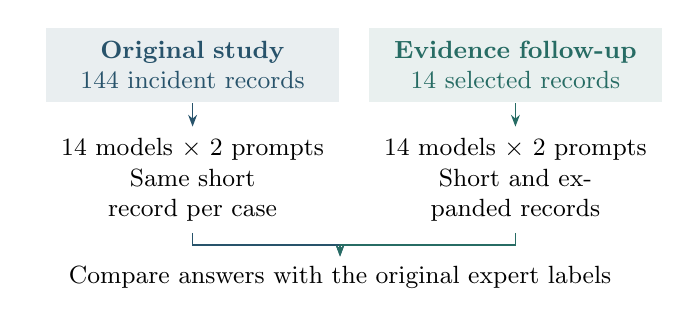
\begin{tikzpicture}[font=\small,box/.style={align=center,text width=3.45cm,minimum height=.95cm,inner sep=4pt},arrow/.style={-{Stealth[length=1.5mm]},line width=.6pt}]
\node[box,fill=studyblue!10,text=studyblue] (a) at (0,0) {\textbf{Original study}\\144 incident records};
\node[box,fill=studyteal!10,text=studyteal] (b) at (4.1,0) {\textbf{Evidence follow-up}\\14 selected records};
\node[box,below=3mm of a] (c) {14 models $\times$ 2 prompts\\Same short record per case};
\node[box,below=3mm of b] (d) {14 models $\times$ 2 prompts\\Short and expanded records};
\draw[arrow,studyblue] (a)--(c);
\draw[arrow,studyteal] (b)--(d);
\node[align=center,text width=7.7cm,below=3mm of c.south east,anchor=north] (e) {Compare answers with the original expert labels};
\draw[arrow,studyblue] (c.south)--++(0,-.15)-|(e.north);
\draw[arrow,studyteal] (d.south)--++(0,-.15)-|(e.north);
\end{tikzpicture}
\Description{Two separate experiments compare model answers with the original expert labels: 144 short records under two prompts, and 14 selected records under both prompts with short and expanded evidence.}
\caption{The two comparisons. The expert consulted extra sources for 14 original cases. The follow-up compares model answers under two evidence conditions against the unchanged expert reference.}
\label{fig:study}
\end{figure}

\section{Legal Framework and Study Scope}
We interpret the results against the July 2024 Act~\cite{aiact2024}: 113 numbered articles, 13 chapters and 13 annexes, covering risk categories, operator duties, governance and enforcement (Supplement S4). Our rubric asks:

\begin{enumerate}
\item \textbf{Is it an AI system?} Art.~3(1) requires an inferential system. Deterministic logging or human analysis alone does not establish this.
\item \textbf{Is the practice prohibited?} Art.~5 lists prohibited practices, each with legal elements to establish. Art.~5(1)(a), for example, concerns manipulative or deceptive techniques, impairment of informed decisions and significant harm or its likelihood.
\item \textbf{Is the system high-risk?} Art.~6 provides two routes. The product route requires a relevant Annex~I product or safety-component role and third-party conformity assessment. The other route covers the listed Annex~III uses, subject to Art.~6(3). That exception cannot apply to profiling.
\item \textbf{Do transparency duties apply?} Art.~50 sets transparency obligations for certain uses, including direct interaction and synthetic content. These duties can also apply to high-risk systems.
\end{enumerate}

The rubric prioritises one summary label: prohibited, high, transparency or minimal. These are not four mutually exclusive harm levels in the Act. We record Art.~50 separately and allow not-AI and insufficient-information answers. ``Minimal'' means no higher rubric category, not harmless or free of legal duties.

The rubric and checklist ask about hypothetical EU placement or use, setting aside territorial and temporal applicability. The basic prompt does not repeat that assumption. Labels are not findings of liability for the reported incidents.

The rubric and checklist also say ``today'', without fixing a legal version. July 2026 amendments added intimate-material prohibitions, product provisions and an annex~\cite{omnibus2026}. Our historical legal framework is an interpretive scope, not a controlled legal-version experiment. Supplement S13 screens potentially affected records; it does not establish current-law accuracy.

Harm alone does not determine the category, although it matters to tests in Arts.~5 and 6(3). Nor does using a general-purpose tool automatically exempt an actor from Art.~5. Commission guidance covers both deployers and general-purpose systems~\cite{commission2025}. Some recorded rubric decisions rely on a narrower view of such misuse; Section~5 explains why those judgments need further review.

\section{Data and Methods}
\subsection{Records and Expert Labels}
We sampled 150 of the 1,618 records with titles and descriptions in the 10 August 2026 AIID export (seed 2026). Keywords in titles, descriptions and party fields assigned records to eight Annex~III-related buckets or a control pool, resolving ties in a fixed domain order. We drew up to 13 per domain and filled remaining places from the control pool. Buckets encouraged variety without establishing legal labels or coverage.

Six development examples were excluded: S019, S026, S028, S041, S059 and S067. Their notes concern employment, recommendation/moderation, migration, benefit decisions and electoral-purpose boundaries. Selection was not documented as random; the examples do not cover all prohibitions or validate the product route. The original 44 \texttt{dev}/106 \texttt{heldout} split becomes 42/102. This pooled evaluation includes development records and later rubric revisions.

The 144 evaluation records span 2012--2026. Descriptions have a median of 358 characters (range 64--599). Models received the year, title, description, developer, deployer and harmed parties, without the sampling bucket or web access.

The first author, a lawyer, developed the rubric and labelled the records. These are his expert assessments of the legally correct categories under the stated interpretation and available evidence. Records include six rule decisions, a category, confidence and notes. The correction log lists 19 field changes across ten incidents. The rubric therefore changed during annotation. The author confirms that these revisions preceded his inspection of model answers. No second expert reviewed the labels; inter-annotator agreement was not measured~\cite{artstein2008}.

The final labels are 77 transparency, 44 high, ten prohibited, nine minimal, two not-AI and two insufficient-information. For 14 records, the expert also consulted full pages or linked reports. We report both the full sample and the remaining 130 records to examine this evidence mismatch. Nine of the excluded records are high-risk, so exclusion also changes the category mix.

\subsection{Prompts and Measures}
Each model received a basic prompt and a longer checklist requesting intermediate rule decisions. Both required a category and short explanation. Legal instructions, scope framing, abstention rules, length and answer structure differed. We compare complete prompts, without isolating a reasoning mechanism.

The checklist's Art.~5(1)(b) summary omits the behaviour-distortion and significant-harm thresholds. Other interpretive assumptions are audited in Supplement S15. Agreement with the archived instruction does not validate its legal completeness.

We use one retained output per model, record and prompt from the original OpenRouter calls: default sampling, a requested 4,096-token completion limit, and no tools. Of 4,032 intended answers, 4,030 were retained; Gemini~3~Flash refused two basic-prompt cases. Original materials are in the \href{https://github.com/stefankofilovski-lang/category-not-severity}{public repository}; model identifiers, usage-log dates, prompts and input hashes accompany the revision.

Exact agreement is the share of answers matching the expert's label. Macro-F1 gives equal weight to each of the six categories, combining precision and recall within each. Missing answers count as nonmatches and false negatives; undefined category F1 scores count as zero. We also report class-wise scores and confusion matrices. Always answering transparency would give 53.5\% exact agreement and 0.116 macro-F1.

QWK~\cite{cohen1968} accounts for label distributions using the assumed order minimal $<$ transparency $<$ high $<$ prohibited. This is not a statutory harm scale. Missing and auxiliary answers have no ordinal score. Table~\ref{tab:agreement} gives scorable counts; paired changes use each model's records scorable under both prompts.

We resample incidents 10,000 times (seed 20260916), keeping both prompts and all models together, to obtain percentile 95\% intervals~\cite{dror2018}. These hold labels and outputs fixed, excluding uncertainty in legal judgments, repeated calls and a wider model population. Individual model comparisons are descriptive, without multiple-testing claims.

\subsection{Additional-Evidence Comparison}
On 22 September, we reran the 14 additional-source cases under both prompts, using fresh short-record baselines and source-linked expansions. Each model received the same record per condition. Thirteen canonical model identifiers match the archive; Qwen3.8 Max uses a disclosed September replacement. Each model used a fixed provider endpoint, with fallback disabled. Original prompts and defaults were retained, although the requested 4,096-token limit did not uniformly cap billed reasoning.

We kept one attempt per cell, including failures, separate from the original results. The original expert labels were retained as a fixed reference and were not reassessed against the new packets. These packets were assembled for the follow-up and do not reconstruct the original annotation evidence. The comparison therefore measures changes in agreement with an existing legal reference. Intervals resample the 14 incidents across models and conditions (10,000 draws, seed 20260922). Repeated-call variability remains unmeasured.

\section{Results and Disagreement Analysis}
\subsection{What Changed with the Checklist?}
Mean exact agreement rose from 73.2\% to 79.5\%, a paired gain of 6.35 percentage points [2.93, 9.87]. Mean macro-F1 barely changed: 0.606 to 0.604, with a paired change of $-0.002$ [$-0.079$, 0.081]. Exact agreement increased for nine models and fell for five; the median gain was 4.51 points.

QWK rose for nine models and fell for five (Table~\ref{tab:agreement}). The means were 0.424 and 0.498, but the paired change on common scorable records was 0.068 [$-0.007$, 0.143]. That interval includes zero. Negative QWK means agreement below the baseline implied by the label distributions; it does not mean every random classifier would do better.

\begin{table*}[!ht]
\centering
\caption{Agreement with the expert legal reference on 144 incidents. B: basic; S: step-by-step. Exact agreement (\%) and six-label macro-F1 include all records. $n_o$: scorable ordinal pairs for QWK; brackets show 95\% incident-bootstrap intervals.}
\label{tab:agreement}
\setlength{\tabcolsep}{4pt}
\small
\begin{tabular}{@{}lrrrll@{}}
\toprule
& Exact B/S & F1 B/S & $n_o$ B/S & QWK B [95\% CI] & QWK S [95\% CI] \\
\midrule
Gemini 3.7 Flash & 86.8/89.6 & 0.77/0.69 & 140/140 & 0.65 [0.46, 0.81] & 0.70 [0.54, 0.85] \\
Gemini 3 Flash & 82.6/83.3 & 0.54/0.51 & 138/140 & 0.57 [0.38, 0.74] & 0.53 [0.32, 0.73] \\
Gemma 3 27B & 68.8/66.7 & 0.29/0.33 & 140/140 & 0.28 [0.13, 0.45] & 0.31 [0.13, 0.50] \\
GPT-5.2 & 81.2/77.8 & 0.69/0.57 & 139/140 & 0.57 [0.39, 0.74] & 0.48 [0.30, 0.64] \\
GPT-5.6 Luna & 81.2/72.2 & 0.73/0.53 & 137/139 & 0.56 [0.39, 0.72] & 0.30 [0.12, 0.46] \\
GPT-5.6 Sol & 79.2/72.9 & 0.76/0.75 & 139/140 & 0.48 [0.30, 0.65] & 0.37 [0.20, 0.53] \\
Grok 4.6 & 79.2/87.5 & 0.74/0.61 & 139/140 & 0.47 [0.29, 0.64] & 0.67 [0.51, 0.82] \\
Claude Haiku 4.5 & 38.9/75.7 & 0.37/0.52 & 134/138 & -0.07 [-0.15, 0.01] & 0.49 [0.31, 0.66] \\
Kimi K2.5 & 75.7/87.5 & 0.68/0.66 & 139/140 & 0.45 [0.27, 0.61] & 0.65 [0.46, 0.81] \\
Kimi K3 & 76.4/74.3 & 0.53/0.58 & 139/139 & 0.54 [0.38, 0.69] & 0.42 [0.25, 0.59] \\
Qwen 3.8 27B & 77.8/85.4 & 0.65/0.79 & 138/140 & 0.47 [0.30, 0.64] & 0.58 [0.40, 0.74] \\
Qwen 3.8 Max & 79.2/85.4 & 0.78/0.79 & 140/140 & 0.39 [0.20, 0.57] & 0.58 [0.41, 0.75] \\
Claude Sonnet 4.6 & 54.2/76.4 & 0.38/0.51 & 137/140 & 0.24 [0.12, 0.37] & 0.40 [0.21, 0.58] \\
Claude Sonnet 5 & 63.2/78.5 & 0.58/0.62 & 137/140 & 0.32 [0.17, 0.47] & 0.48 [0.31, 0.65] \\
\bottomrule
\end{tabular}
\end{table*}


Excluding the 14 additional-source cases gave exact agreement of 71.7\% and 79.5\%. Mean QWK was 0.379 and 0.469, with a paired change of 0.083 [0.001, 0.166]. This checks sensitivity to the affected cases but cannot undo their original evidence mismatch. Excluding 15 automated-driving cases instead left 129 records and a paired QWK change of 0.059 [$-0.020$, 0.137]. This addresses one recurring case family, not all possible dependence between reports.

On the 102 records marked held-out in the original split, exact agreement increased by 5.32 points [1.47, 9.31]. This post-hoc partition check does not establish an untouched test set (Supplement S13).

\subsection{Did More Evidence Help?}
We attempted all 784 follow-up calls. Of these, 750 returned valid category answers for the requested incident and 34 did not. Expanded records changed 18 of 187 basic-prompt labels and 26 of 179 step-by-step labels among pairs with valid answers in both conditions.

The unweighted mean of model-specific changes on common valid pairs was 0.18 percentage points [$-3.53$, 3.85] under the basic prompt and $-8.95$ [$-15.48$, $-3.23$] under the checklist. Counting failed answers as nonmatches gave $+0.51$ and $-7.14$ points (Supplement S11). New expanded packets did not consistently increase agreement; the scores cannot determine whether changed answers are legally better.

\subsection{Where Did Answers Differ?}
Figure~\ref{fig:revision} separates 109 records labelled outside Annex~III and 33 inside; two unclear cases are excluded from this contrast. Outside Annex~III, mean signed disagreement fell from $+0.24$ to $+0.12$. Inside, it shifted from $-0.02$ to $-0.12$. The signs show direction relative to the expert under the imposed category order. Category mix and the ends of that scale matter: a prohibited reference cannot be over-classified, nor a minimal one under-classified. Supplement S6 also compares answers within each reference category.

The most common basic-prompt confusion was transparency to prohibited: 200 of 1,078 answers on transparency cases, falling to 126 with the checklist. In the other direction, prohibited to transparency rose from 48 to 62 of 140 answers. This helps explain why exact agreement and macro-F1 give different pictures. Domain comparisons are limited by very small counts: education and justice/democracy have one reference incident each, employment has two, and critical infrastructure has none.

\begin{figure*}[!ht]
\centering
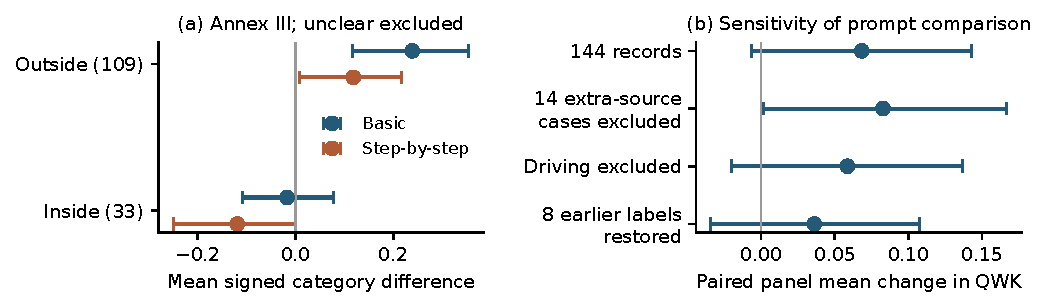
\includegraphics[width=.97\textwidth]{fig_revision.pdf}
\Description{Interval plots show signed category disagreement inside and outside Annex III, and paired prompt differences under four sensitivity analyses.}
\caption{Results with 95\% incident-bootstrap intervals. (a) Signed category disagreement by the expert's Annex~III classification; two unclear cases are excluded. (b) Checklist minus basic QWK on common scorable records. The eight-label check restores documented earlier labels; neither version has independent legal validation.}
\label{fig:revision}
\end{figure*}

Checklist answers matched the expert on Art.~5 in 1,544/2,016 model--incident pairs (76.6\%). Agreement was 1,921 (95.3\%) for the product question, 1,716 (85.1\%) for Annex~III domain, 1,804 (89.5\%) for derogation, 1,705 (84.6\%) for profiling and 1,874 (93.0\%) for transparency. These rates include negatives and not-applicable values; missing steps count as nonmatches. On Art.~5-positive references, agreement was 51/140 (36.4\%; Supplement S14). A first recorded difference does not identify its cause; the basic explanations leave much reasoning unobserved.

Three cases illustrate these differences. S058 describes a fatal incident involving a stacking robot. The expert assigned minimal based on an assumption about product assessment. Twelve basic answers said high and two said not-AI; ten checklist answers said minimal. For S011, facial-image search, ten models under each prompt said prohibited. The expert recorded high because his assessment did not establish untargeted scraping. For S024, activity logs in a cheating investigation, agreement with not-AI fell from eight models to six. The case dossiers include all model labels, contrary explanations and unresolved facts; they are not new human evaluations of the answers.

\section{Discussion and Limitations}
Disagreement can reflect unsupported assumptions, competing legal readings or a reference judgment needing revision. In S083, the expert's note describes deception, age vulnerability and financial harm, while the corrected label is transparency. Each legal element needs assessment; general-purpose use is not a blanket exemption. Supplement S13 also checks sensitivity to 22 fraud-related transparency records.

We tested how much earlier label changes affect the results by restoring eight documented prohibited-to-transparency corrections to their previous categories. Mean QWK became 0.393/0.437, with a paired change of 0.036 [$-0.034$, 0.107]. This tests sensitivity to recorded history without changing the original data or validating either legal interpretation.

Neither the reference labels nor the error interpretations have been independently replicated. The audit followed the model runs. AI helped select and prepare cases; the author made the three recorded legal judgments, retaining S014, S024 and S140. Post-run AI suggestions did not change the expert reference. This is guided case review, not human rating of every model explanation (Supplement S12). Development records and rubric revisions limit independence. The sample does not represent incident prevalence; rare classes make macro-F1 unstable, and short reports omit relevant facts. We did not independently measure incident severity. Category composition could explain the directional pattern. The historical framework limits current-law conclusions.

% Start the final section with the pending results figure; balance this page only.
\newpage
\balance
\section{Conclusion}
A legal checklist increased average exact agreement with the expert, but the benefit varied by model and measure. Additional source evidence did not consistently improve agreement. The practical lesson is to report the evidence, rubric and disputed judgments alongside the scores. Independent legal review is still needed before extending these findings to broader claims of legal accuracy.

\begin{acks}
The research was supported through the European project Raido (GA 101135800). LLM assistance was used for manuscript editing, analysis code, source-packet preparation, and selecting and preparing post-run review cases. The authors are responsible for checking the calculations, legal interpretations and final text.
\end{acks}
\printbibliography
\end{document}
% All numbers below are preserved from the independently checked baseline.
